\chapter{Исследовательская часть}

В данном разделе будут приведены примеры работы программ,
постановка эксперимента и сравнительный анализ алгоритмов на основе
полученных данных.

\section{Технические характеристики}

Технические характеристики устройства, на котором выполнялось тестирование,
следующие.

\begin{itemize}
	\item Операционная система: macOs Monterey 12.4\cite{ubuntu}.
	\item Память: 16 Гбайт.
	\item Процессор: 2,6 ГГц 6‑ядерный процессор Intel Core i7\cite{intel}.
\end{itemize}

Тестирование проводилось на ноутбуке, включенном в сеть электропитания.
Во время тестирования ноутбук был нагружен только встроенными приложениями
окружения, а также непосредственно системой тестирования.


\section{Время выполнения алгоритмов}

В таблице \ref{tab:time0} представлены замеры времени работы для каждого из алгоритмов для квадратных матриц небольшого размера (1-9). Здесь и далее: СА — стандартный алгоритм, АВ — алгоритм Винограда, ОАВ -- оптимизированный алгоритм Винограда. Время в микросекундах.

\begin{table}[h]
	\begin{center}
		\captionsetup{justification=raggedright,singlelinecheck=off}
		\caption{\label{tab:time0}Результаты замеров времени алгоритмов (миллисекунды)}
		\begin{tabular}{|c|c|c|c|c|}
		\hline
		Размер & СА &  АВ & ОАВ \\
		\hline
		10  & 57 & 48 & 29\\
		\hline
		50  & 5764 & 3996 & 2161\\
		\hline
		100  & 38218 & 25298 & 13236 \\
		\hline
		200  & 290076 & 201203 & 107843 \\
		\hline
		300  & 974186 & 791162 & 434455 \\
		\hline
		400  & 2645162 & 1833453 & 1174284 \\
		\hline
		500  & 5143356 & 3717723 & 2208044 \\
		\hline
		\end{tabular}
	\end{center}
\end{table}

Также наглядной иллюстрацией зависимости времени выполнения от размера матрицы является график \ref{gra:rand}.
\begin{figure}[h!]
	\centering
	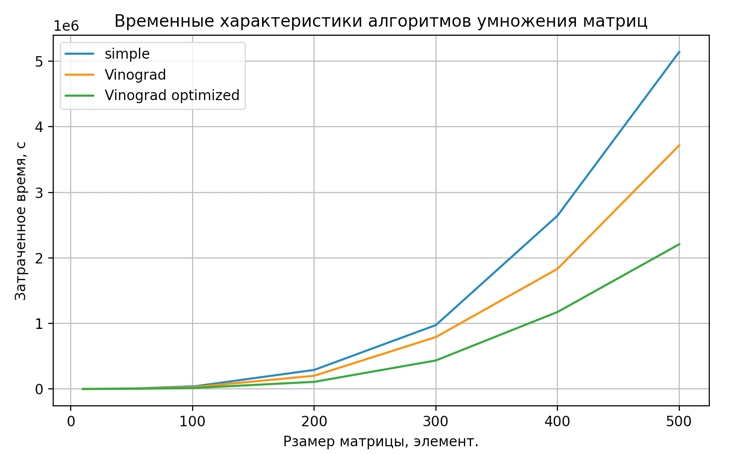
\includegraphics[width=1\linewidth]{img/graph.png}
	\caption{График зависимости времени выполнения влгоритма от размеров квадратной матрицы)}
	\label{gra:rand}
\end{figure}
\newpage

\section*{Вывод}
При увеличении размера матриц, увеличивается и эффективность работы алгоритма Винограда в сравнении со стандартным алгоритмом. В среднем реализация по Винограду работает быстрее в 1.7 раз. Оптимизированная реализация алгоритма Винограда также позволяет уменьшить время работы при больших размерностях: например, для размерности матрицы, равной 200, эксперимент показал, что алгоритм Винограда быстрее стандартного алгоритма чуть менее, чем в 2 раза, когда оптимизированная версия выигрывает у обычного умножения более, чем в 2 раза. 
